\chapter{High-speed data transmission}

\section{Introduction}

While sensors can capture both still images and video, this project focuses on the latter due to its resource-intensive nature. A recent study found that 75\% of households in the United States had a high-definition television \cite{14_leichtman_research_group_2013}. The popularity of HD content makes it important to consider how throughput requirements increase with larger resolutions. An uncompressed 24-bit colour 1080p video at 60p has a bitrate of almost \SI{3}{\giga\bit\per\second}, as calculated in Equation \ref{eq:hd_throughput}, well within the range where signal integrity becomes important.

\begin{equation}
  \begin{split}
    \mathbf{BW} &= (1920*1080) \, \mathrm{pixels} * 24  \, \mathrm{bpp} * 60 \, \mathrm{fps} \\
                &= 2.99  \, \mathrm{Gbits/s}
  \end{split}  
  \label{eq:hd_throughput}
\end{equation}

When transmitting a high-frequency signal between two devices, close attention must be paid to many aspects of the design to ensure that the signal integrity is preserved. The basic premise of high-speed design is covered here. With low-frequency signals, a wire or PCB trace can be modelled as an ideal circuit, without resistance, capacitance or inductance. As the frequency increases however, so-called transmission line effects are prominent and the \gls{ac} characteristics of the wire become very important. If there is a mismatch between the source, line and receiver impedances then the transmitted signal will not be fully absorbed at the load, resulting in any excess energy rebounding between source and receiver repeatedly until it has been fully absorbed. Due to superposition, the reflected waves will cause ringing and other signal integrity issues that reduce signal quality. If the issue is severe enough, the receiver cannot correctly interpret the signal and bit errors will occur. Parallel wires can also cause mutual inductance problems whereby the magnetic field generated by current travelling through one wire, will induce a current in the adjacent wire. This mutual inductance, along with the increased cost and complexity arising from wide parallel busses, are why serial interfaces are typically preferred for high-speed designs. Similarly, mutual capacitance is caused by the coupling of the two electric fields. These issues can be mitigated by taking care to ensure that impedance is properly controlled and \gls{pcb} traces are placed with care when designing circuits \cite{15_basic_principles_of_signal_integrity_2007}.

\section{Basic considerations for high-speed interface design}

\subsection{Differential signalling}

When considering the signal path of a board-to-board interface, the possibility of signal degradation from external interference becomes obvious: signals must travel from drivers on the transmitter chip, across the board to a connector, over some sort of medium connecting the two boards, through another connector on the second board and into a buffer on the receiver chip. Electromagnetic interference can cause noise in the transmission medium which will have an adverse effect on a single-ended system by ultimately increasing the \gls{ber}. In contrast, differential systems provide better noise immunity because any common-mode noise is cancelled out when the two signals are subtracted.

\subsection{SerDes}
\gls{fpga} designs always have a maximum operating frequency which dictates how fast data can be reliably clocked into the flip-flops. When using the global clock network, the Xilinx Zynq-7010 \gls{fpga} used in this project has a theoretical maximum internal frequency of \SI{710}{\mega\hertz}, denoted by \(F_{MAX\_BUFIO}\)\cite{xilinx:ds187}. A problem becomes immediately obvious: the internal logic in the \gls{fpga} is not fast enough to clock out data at the required throughput calculated in Equation \ref{eq:hd_throughput}. To mitigate this, many \glspl{fpga} allow the \gls{io} clocks to switch much faster than the rest of the fabric. Direct access to the pins at these high frequencies is not possible, however each \gls{iob} contains a \gls{serdes} block which can be used to obtain the maximum theoretical throughput. Fundamentally they act like high-speed parallel-serial and serial-parallel converters. A serialiser block is used to take an \(n\)-bit input signal and transmit it bit-by-bit over a single line at \(n\)-times the input rate. At the other end of the link, the deserialiser clocks the data in and outputs an \(n\)-bit signal every \(n\) clock cycles. A simplified \gls{serdes} pair is illustrated in figured \ref{fig:serdes_diagram}.

\begin{figure}
  \centering
  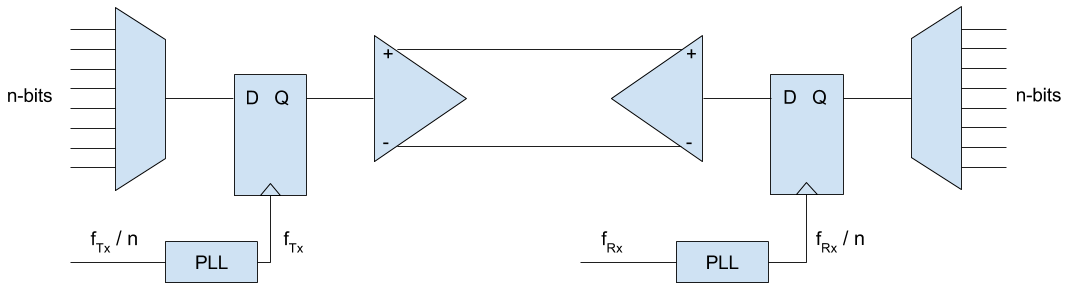
\includegraphics[width=1\textwidth]{./img/serdes.png}
  \caption{Simplified diagram of an n-bit serialiser and deserialiser pair.}
  \label{fig:serdes_diagram}
\end{figure}

By using \gls{serdes}, achieving the required throughput from Equation \ref{eq:hd_throughput} seems much more feasible. In fact modern \glspl{fpga} contain multi-gigabit transceivers which far surpass the throughput required for 1080p video transmission.

\subsection{Line encoding}
Before the data is sent onto the line it is normally run through a line coding scheme which turns the data bits into a form which is more suitable for the receiver to decode. A typical example would be the 8b10b line coding scheme, which turns \SI{8}{\bit} of data into a \SI{10}{\bit} word which has certain properties. The line coding scheme is designed to change several properties of the data such as eliminating any \gls{dc} offset. For example, a run of 100 ones followed by a zero would have a very obvious positive \gls{dc} offset --- this would cause problems in a wireless system where transmission relies on \gls{ac} signals. Some line coding schemes will modify the data to include as many transitions as possible so that the clock can be recovered at the receiver and used to decode the incoming bitstream. Transitions unfortunately have the side effect of radiating a considerable amount of electromagnetic noise. For systems where the clock is transmitted separately it may be desirable to instead minimise the number of transitions to reduce the amount of \gls{emi} produced. The line coding scheme must ensure though that each input word maps to a unique output word --- no two inputs should produce the same output.

Because the receiver is clocked by the transmitter it is important to ensure both sides are properly synchronised. As it is possible to start decoding part way through a word, the line coding scheme uses special control characters (named commas) to indicate periods of synchronisation and mark the boundary between symbols. Upon detecting a comma, the receiver is able to phase-shift the signal until it is properly aligned. 

\section{Analysis of existing camera and video interfaces}
\textit{Not invented here syndrome} is common in the technology field, however there are numerous reasons to adopt an existing interface: prior use guarantees a certain level of field testing, increasing reliability. Using an existing interface can reduce development costs and time-to-market, however due care must be paid to licensing, which can potentially lead to higher costs than developing a custom interface from scratch. Existing interfaces likely increase adoption rates among third-party developers creating their own image sensor modules and cameras – using an interface which they already have experience with is more attractive than the learning-curve associated with understanding a new interface. Having third-parties invest into such an interface by creating products for it is absolutely key to ensuring a thriving ecosystem.

\begin{table}
  \centering
  \begin{tabular}{llllll}
  Name      & Parent  & Family    & Bandwidth & Scheme  & Complexity \\
  \hline
  USB3 Vision   & USB 3   & USB       & 2.8 Gbps  & Serial  & High \\
  GigE Vision   & IP / UDP  & Ethernet    & 800 Mbps  & Serial  & Medium \\
  Camera Link   & N/A     & Camera Link   & 6.8 Gbps  & Serial  & Medium \\
  MIPI CSI-3  & M-PHY   & MIPI      & 23.2 Gbps & Serial  & Medium \\
  HDMI 2.0    & N/A     & HDMI      & 18 Gbps   & Serial  & Low / Medium \\
  DVI 1.0     & N/A     & DVI       & 3.96 Gbps & Serial  & Low \\
  DisplayPort 1.2 & N/A   & DisplayPort   & 
  \end{tabular}
  \caption{Existing protocols and interfaces for transmitting image data      \protect\cite{16_von_fintel_2013,17_arrowdevices.com_2014,18_hdmi.org}}.
  \label{table:existing_protocols}
\end{table}

Table \ref{table:existing_protocols} shows a list of popular video interfaces / protocols in widespread use today. Bandwidth is by far the most important metric when choosing an interface as it needs to be able to accommodate a 1080p RAW video stream. Equation \ref{eq:hd_throughput} calculated the required bandwidth for the RGB image format, however adjustments are required for the RAW image format, which only has a single channel used to store pixel intensities. 

\begin{equation}
  \begin{split}
    \mathbf{BW} &= (1920*1080) \, \mathrm{pixels} * 8  \, \mathrm{bpp} * 60 \, \mathrm{fps} \\
                &= 0.995  \, \mathrm{Gbits/s}
  \end{split}  
  \label{eq:1080p_raw_throughput}
\end{equation}

Equation \ref{eq:1080p_raw_throughput} calculates the bandwidth required by a 1080p RAW video stream to be \SI{~1}{\giga\bit\per\second}, which makes sense given only a single channel is used, as opposed to the three required for the RGB format. With the exception of GigE Vision, all of the interfaces in Table \ref{table:existing_protocols} have sufficient bandwidth for 1080p RAW video. GigE Vision is a special case because the bandwidth is limited by the underlying physical layer protocol, which in this case is Gigabit Ethernet. Because of how GigE Vision fits into the TCP / IP stack, it is trivial to swap the physical layer for something faster like 10 Gigabit Ethernet, 10GbE transceivers are only typically found in high-end FPGAs which are prohibitively expensive.

Licensing requirements play a critical role in the choice of interface. While there is no concrete definition for what constitutes an open standard, OpenStand (an interest group formed by IEEE, ISOC and W3C) states that open standards are those 'that can be implemented under fair terms. Given market diversity, fair terms may vary from royalty-free to fair, reasonable, and non-discriminatory terms' \cite{open_standard_definition}. USB3 Vision, GigE Vision and Camera Link and HDMI all require the payment of a licence fee, while MIPI CSI-3 requires MIPI Alliance membership in order to access the specifications. \gls{dvi} (created by the Digital Display Working Group) has a freely-available specification and is royalty-free, however DDWG membership is required in order to use the \gls{dvi} logo and list official compliance. DisplayPort is also royalty-free.

None of the existing interfaces have everything required for an image sensor interface and so it is essential that the specification allows for some amount of extension in order to accommodate these features. Ideally, the interface should allow for this to be done in such a way so as not to break the interface's specification. Packet-based protocols such as DisplayPort and USB3 Vision are ideal for this because custom packet types which co-exist with the rest of the protocol can be created for these extensions.

\subsection{Using \gls{dvi} as the basis for an image sensor interface}
Despite its age, \gls{dvi} is still a capable interface. The combination of royalty-free licensing, simplicity and bandwidth capabilities make it an ideal choice as the basis for transferring image sensor data. While DisplayPort is arguably more future-proof in terms of bandwidth capabilities and extensibility, it comes at the cost of increased complexity due to the packet-based nature of the protocol. Furthermore, while \gls{dvi} includes blanking periods similar to legacy interfaces such as VGA, this can actually be used to our advantage when extending the interface, as we will see in later sections. In addition to the reasons above, \gls{dvi} has several other attractive options such as:

\begin{itemize}
  \item{One can add custom extensions into blanking period without breaking spec}
  \item{No complex clock recovery}
  \item{I\textsuperscript{2}C lines for custom configuration and firmware updates}
  \item{\gls{edid} to advertise capabilities}
  \item{Hot plug detection}
\end{itemize}